% !TEX program = xelatex
% 공통수학2 · Ⅱ. 집합과 명제 · 1. 집합 · 01 집합 · 2/2차시
% 학생용 활동지 (답안 없음)
\documentclass[11pt,a4paper]{article}
\usepackage{kotex}
\usepackage{iftex}
\ifPDFTeX\else
  \setmainhangulfont{Noto Serif CJK KR}
  \setsanshangulfont{Noto Sans CJK KR}
\fi
\usepackage[margin=2.1cm]{geometry}
\usepackage{parskip}
\usepackage{enumitem}
\usepackage{array}
\usepackage{tabularx}
\usepackage{xcolor}
\usepackage{amssymb}
\usepackage{tikz}
\usepackage[most]{tcolorbox}
\usepackage{fancyhdr}
\usepackage{titlesec}

\definecolor{goldc}{HTML}{B07C22}
\definecolor{goldstrong}{HTML}{8A5F16}
\definecolor{indigoc}{HTML}{2B3B57}
\definecolor{indigosoft}{HTML}{6E82A6}
\definecolor{linec}{HTML}{D6DACB}
\definecolor{surface2}{HTML}{E4E8DC}
\definecolor{writeline}{HTML}{C7CCBA}
\definecolor{inksoft}{HTML}{52604F}

\titleformat{\section}{\normalfont\sffamily\bfseries\large\color{indigoc}}{\thesection}{0.6em}{}
\titlespacing{\section}{0pt}{14pt}{6pt}
\newtcolorbox{goalbox}{enhanced, breakable, colback=white, colframe=goldc, boxrule=0.5pt, leftrule=3pt, arc=2pt, left=10pt, right=10pt, top=8pt, bottom=8pt}
\newtcolorbox{sheetbox}{enhanced, breakable, colback=white, colframe=linec, boxrule=0.6pt, arc=3pt, left=11pt, right=11pt, top=9pt, bottom=9pt}
\newcommand{\writespace}[1]{%
  \par\nobreak\vspace{3pt}
  \foreach \n in {1,...,#1} {%
    \noindent\textcolor{writeline}{\rule{\linewidth}{0.4pt}}\par\vspace{0.62cm}%
  }
}
\newcommand{\fillblank}[1]{\makebox[#1]{\hrulefill}}
\pagestyle{fancy}\fancyhf{}\renewcommand{\headrulewidth}{0pt}
\fancyfoot[L]{\footnotesize\color{inksoft} 공통수학2 · 2026학년도 2학기 · 지평선고등학교}
\fancyfoot[R]{\footnotesize\color{inksoft} 다음 시간 --- 02 집합 사이의 포함 관계}

\begin{document}

\noindent
\begin{minipage}[b]{0.62\linewidth}
  {\sffamily\footnotesize\color{indigosoft} 공통수학2 · Ⅱ. 집합과 명제 · 1. 집합}\\[2pt]
  {\sffamily\bfseries\Large 01 집합 \textperiodcentered\ 19차시}
\end{minipage}\hfill
\begin{minipage}[b]{0.36\linewidth}
  \raggedleft\small\color{inksoft}
  반\ \fillblank{1.6cm} \quad 번호\ \fillblank{1.6cm}\\[4pt]
  이름\ \fillblank{3.6cm}
\end{minipage}

\vspace{4pt}
\noindent{\color{goldc}\rule{\linewidth}{2.2pt}}
\vspace{10pt}

\begin{goalbox}
\textbf{오늘의 목표}\\
집합을 벤 다이어그램으로 나타내고, 유한집합·무한집합·공집합을 구분하며 원소의 개수를 구할 수 있다.
\vspace{4pt}
\small\color{inksoft}
$\square$ 자신 있음 \quad $\square$ 조금 헷갈림 \quad $\square$ 처음 봄 \hfill (수업 전 나의 상태에 표시)
\end{goalbox}

\section{생각 열기 --- 벤 다이어그램으로 그려보기}

\begin{sheetbox}
집합 $A=\{a,b,c,d,e\}$를 벤 다이어그램으로 그려 보자.

\vspace{4pt}
\begin{center}
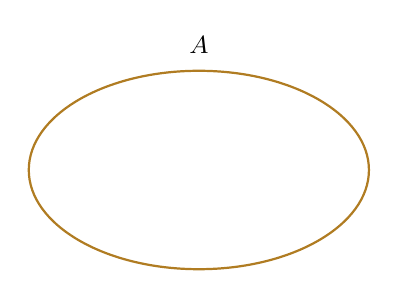
\begin{tikzpicture}[scale=0.9]
  \draw[thick, goldc] (0,0) ellipse (2.4 and 1.4);
  \node[above, font=\small] at (0,1.5) {$A$};
\end{tikzpicture}
\end{center}

원소가 하나도 없는 집합은 벤 다이어그램으로 어떻게 그리면 좋을지 생각해서 오른쪽 빈 원 안에 표시해 보자.
\writespace{2}
\end{sheetbox}

\section{개념 정리 --- 원소의 개수}

\begin{sheetbox}
원소가 유한개인 집합을 \fillblank{2.6cm}, 원소가 무수히 많은 집합을 \fillblank{2.6cm}이라고 한다. 집합 $A$가 유한집합일 때, 원소의 개수를 기호로 $n(A)$와 같이 나타낸다.

\vspace{6pt}
원소가 하나도 없는 집합을 \textbf{공집합}이라 하며, 기호 $\varnothing$으로 나타낸다. 공집합은 $n(\varnothing)=\fillblank{1.2cm}$인 유한집합으로 생각한다.

\vspace{10pt}
\textbf{생각해보기} --- 집합 $\{0\}$은 공집합일까? 이유를 적어 보자.
\writespace{2}
\end{sheetbox}

\section{연습 문제}

\begin{sheetbox}
\textbf{1.} 집합 $B=\{x\mid x$는 $|x|\le2$인 정수$\}$를 벤 다이어그램으로 나타내시오.
\writespace{3}

\vspace{6pt}
\textbf{2.} 다음 집합 $A$에 대하여 $n(A)$를 구하시오.\\
\hspace*{1.6em}⑴ $A=\{3,6,9\}$\\
\hspace*{1.6em}⑵ $A=\{1^2,2^2,3^2,\dots,10^2\}$\\
\hspace*{1.6em}⑶ $A=\{x\mid x^2=-4$인 실수$\}$\\
\hspace*{1.6em}⑷ $A=\{x\mid x^2-2x-3=0\}$
\writespace{5}
\end{sheetbox}

\section{사고의 가시화 --- Connect · Extend · Challenge}

\noindent{\footnotesize\color{inksoft} `집합' 전체(18$\sim$19차시)를 떠올리며 아래 세 칸을 채워 보자.}\\[6pt]
\begin{tabularx}{\linewidth}{@{}XXX@{}}
\textbf{\footnotesize\color{indigoc} Connect --- 무엇과 연결되나?} &
\textbf{\footnotesize\color{indigoc} Extend --- 어디까지 확장됐나?} &
\textbf{\footnotesize\color{indigoc} Challenge --- 아직 궁금한 것은?} \\[4pt]
\end{tabularx}
\noindent
\begin{minipage}[t]{0.32\linewidth}\writespace{3}\end{minipage}\hfill
\begin{minipage}[t]{0.32\linewidth}\writespace{3}\end{minipage}\hfill
\begin{minipage}[t]{0.32\linewidth}\writespace{3}\end{minipage}

\section{마무리 성찰}

\begin{sheetbox}
\begin{minipage}[t]{0.48\linewidth}
{\footnotesize\color{inksoft} `집합' 소단원을 마치며 한 문장으로}
\writespace{2}
\end{minipage}\hfill
\begin{minipage}[t]{0.48\linewidth}
{\footnotesize\color{inksoft} 감사 일기 / 유념 한 줄}
\writespace{2}
\end{minipage}
\end{sheetbox}

\end{document}
